\section{Tests préliminaires}
Le but des tests préliminaires est de vérifier que les analyses effectuées dans la phase de recherche sont applicables et nous retournent
des résultats exploitables. Ils permettent également de se rendre compte si le système imaginé lors de la sélection du matériel est en accord avec
ce qui est réalisable.
\subsection{Matériel}
Au moment des tests, les élements suivants étaient à ma disposition :
\begin{itemize}
    \item 1x Rapsberry Pi 4b - 4Go de RAM.
    \item 1x Pi caméra module 3 NoIR Wide.
    \item 20x leds IR 830nm.
    \item 20x leds IR 850nm.
    \item 20x leds IR 880nm.
    \item 1x morceau de route.
    \item 1l. Huile de moteur neuf - 15W-40.
\end{itemize}

\subsection{Eclairage}
L'éclairage utilisé dans le cadre des tests préliminaires consiste en deux rails de leds IR montées en ligne sur deux veroboards.
Le montage a été effectué selon le schéma suivant:
\begin{figure}[H]
    \centering
    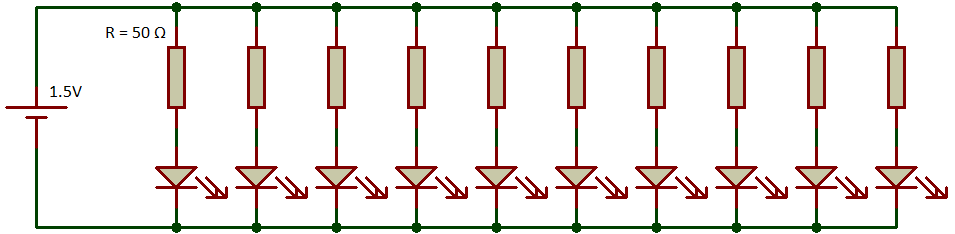
\includegraphics[width=13cm]{assets/figures/schema_leds1.png}
    \caption{Eclairage de test - Schéma électrique de la rangée de led - Schéma modifié de: https://www.sonelec-musique.com/electronique_realisations_alim_led.html}
\end{figure}
Les veroboards sont pratiques à manipuler, il est possible se les tenir avec des étaux afin de faire varier les positions durant les tests. Une fois monté,
le résultat est le suivant:
\begin{figure}[H]
    \centering
    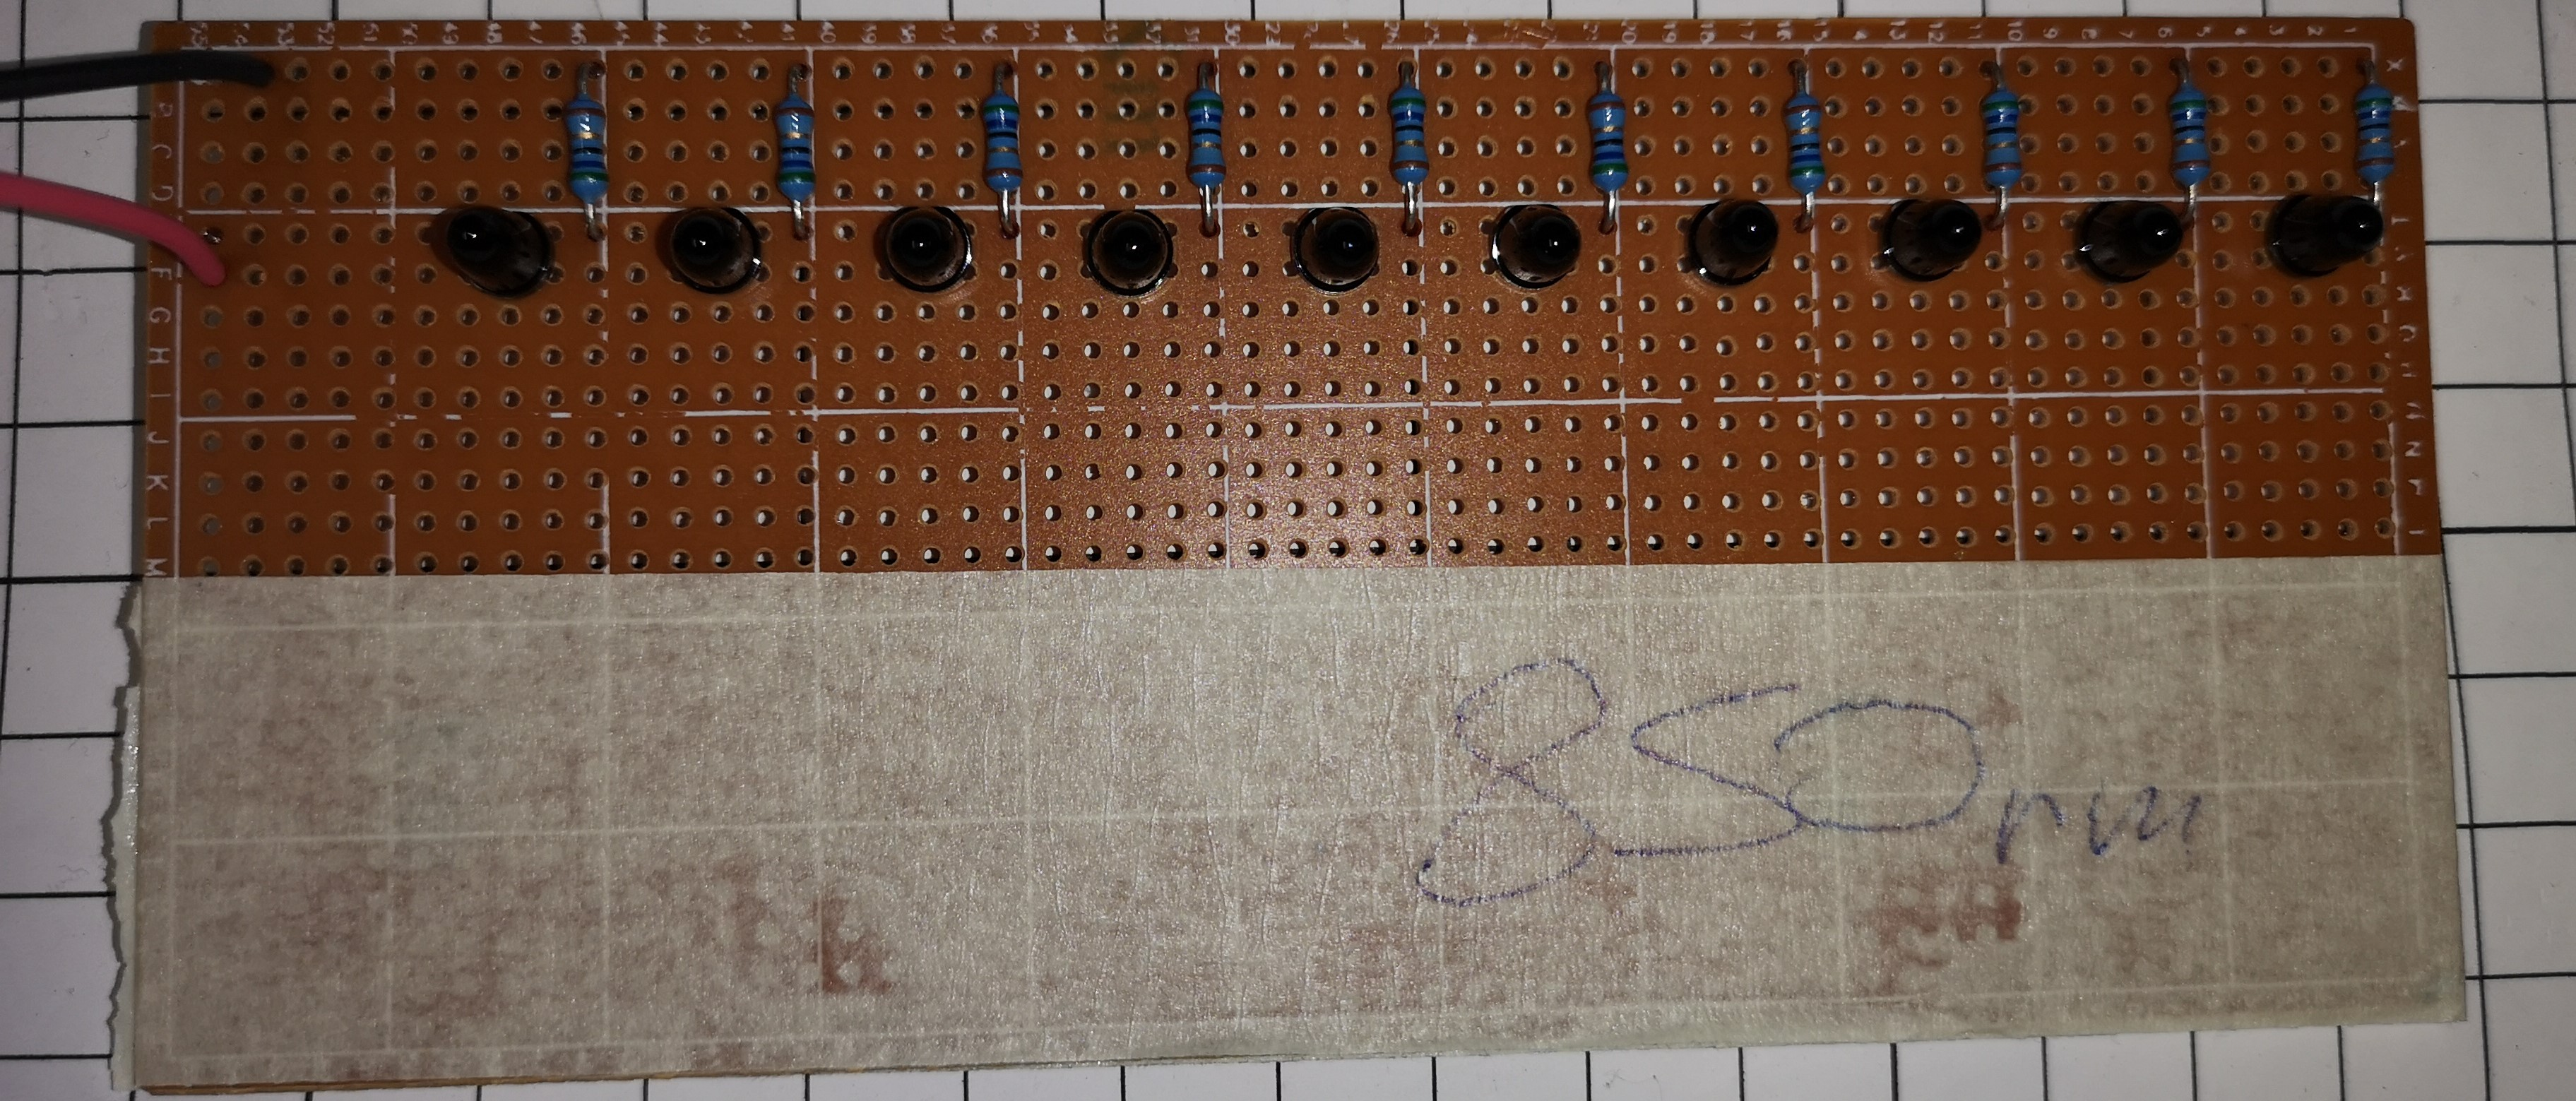
\includegraphics[width=13cm]{assets/figures/rail_led1.jpg}
    \caption{Eclairage de test - Rail de leds 1}
\end{figure}

\begin{figure}[H]
    \centering
    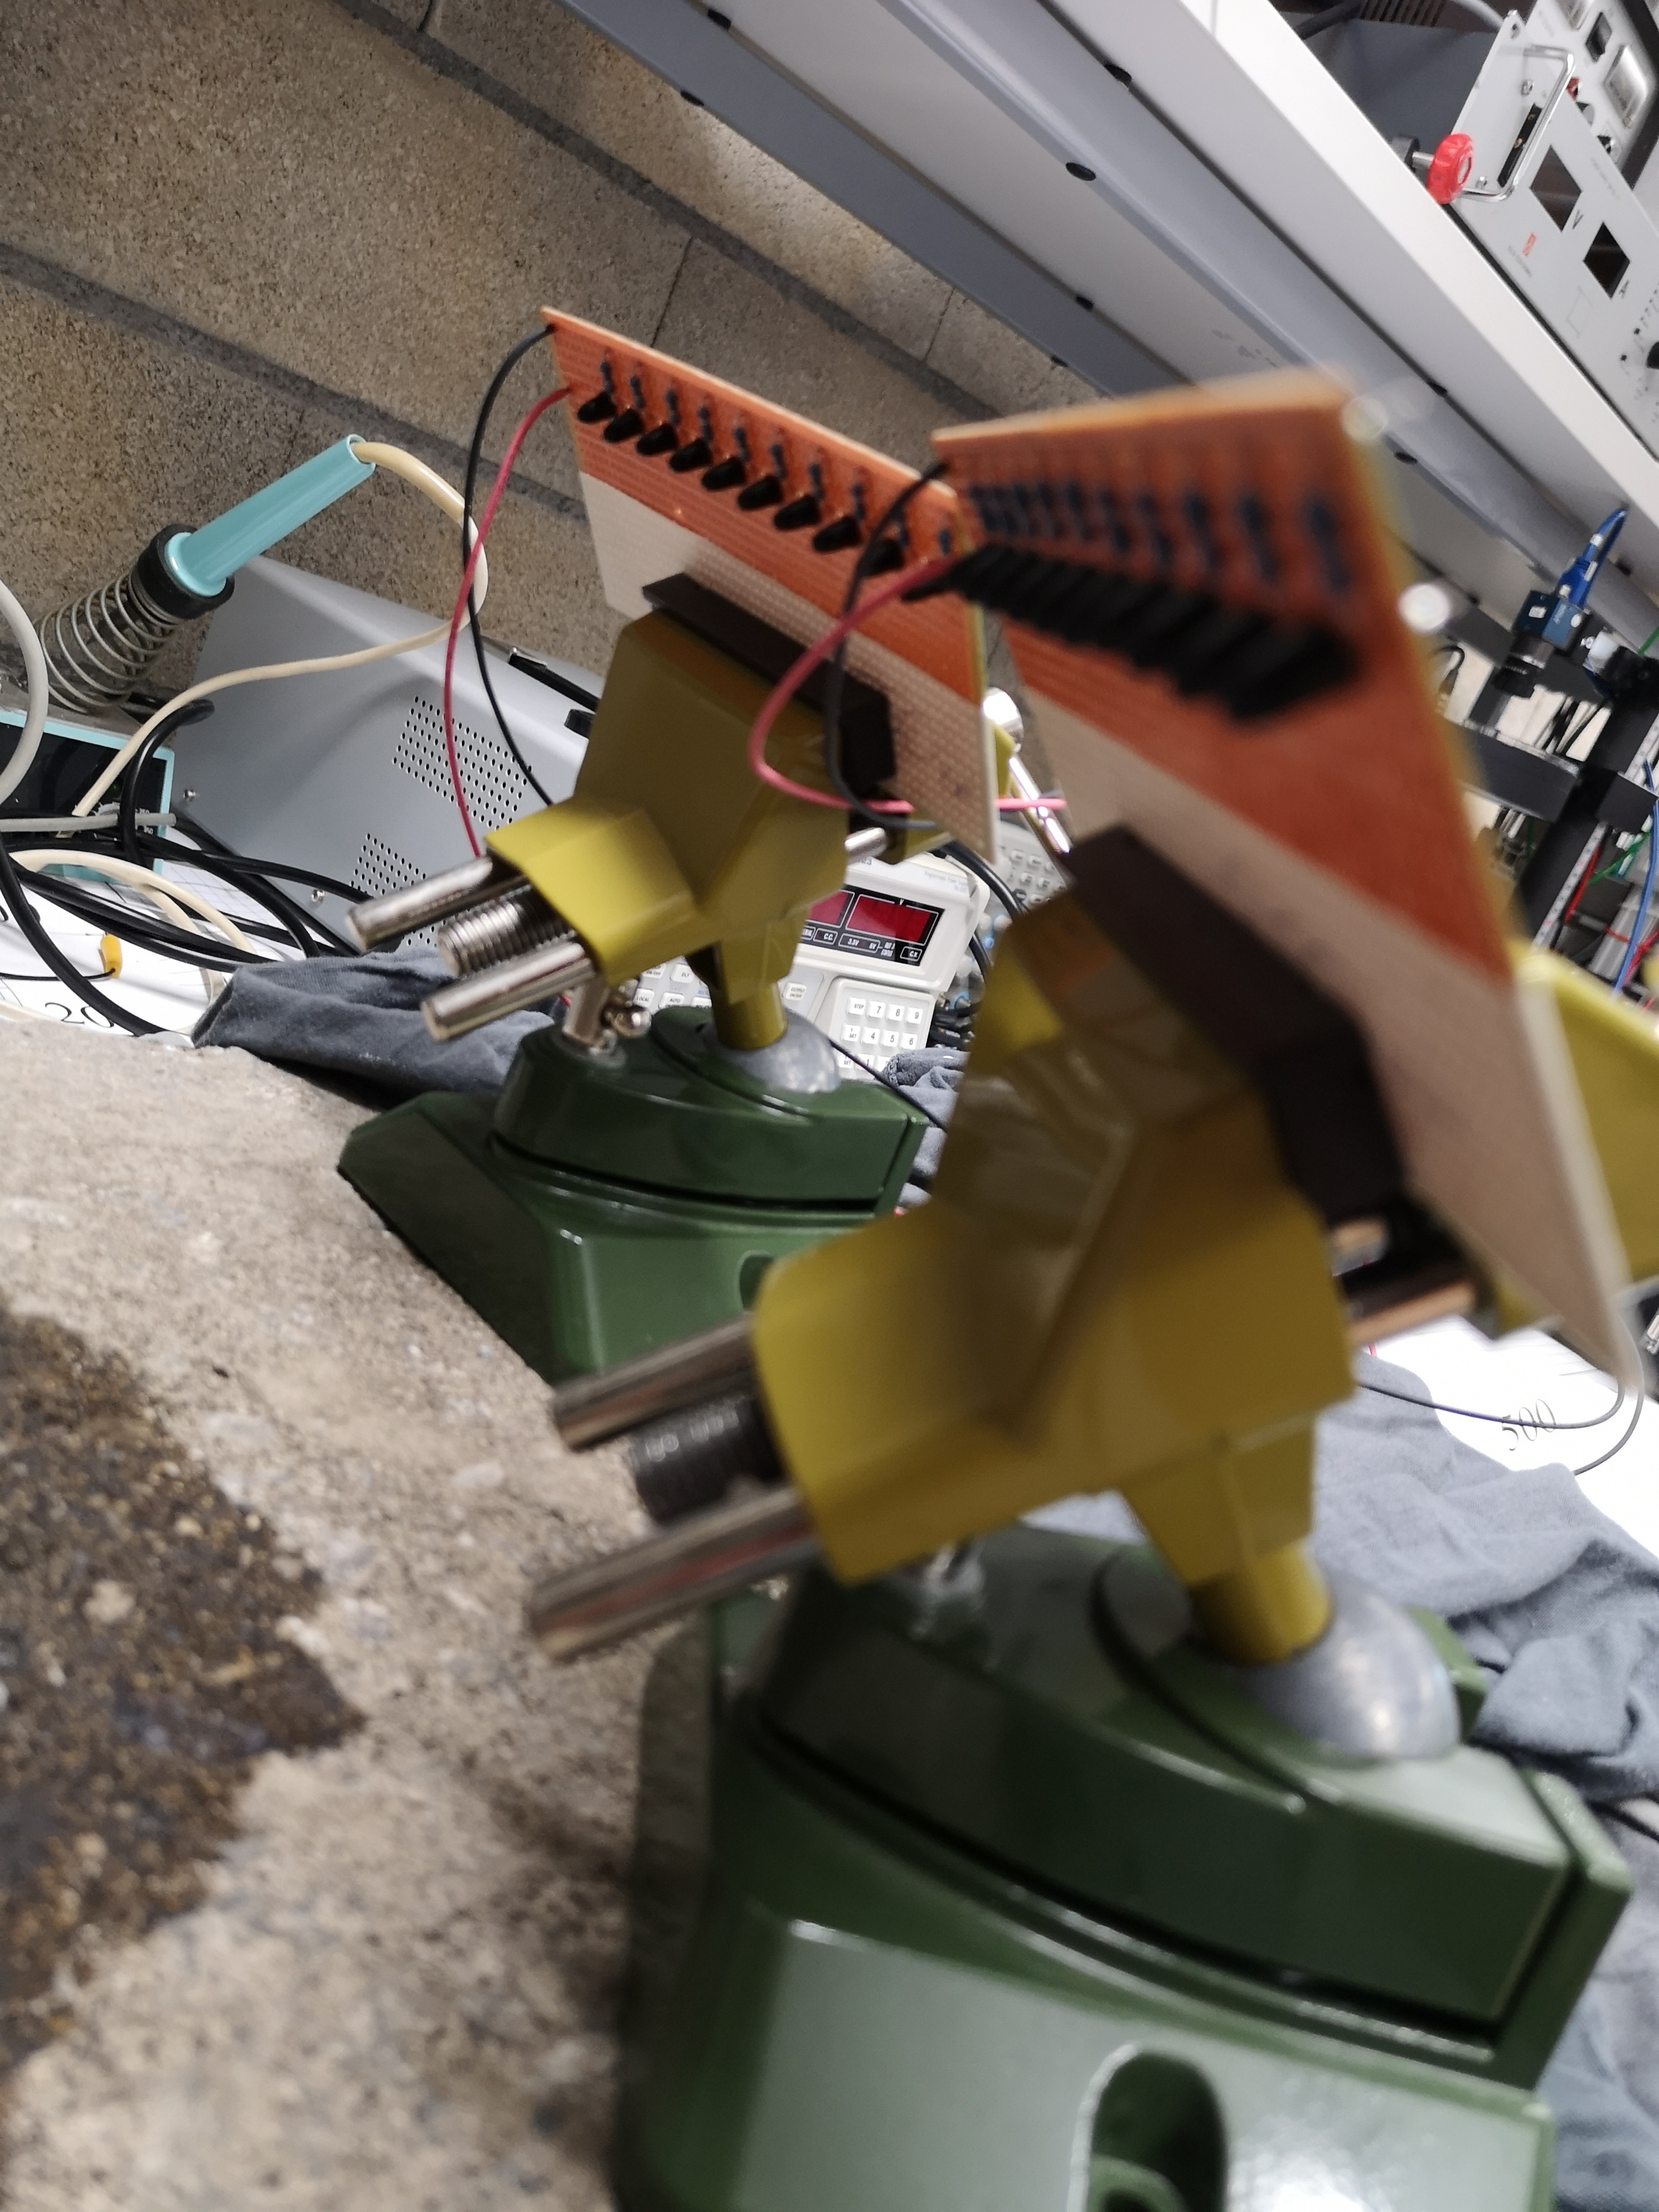
\includegraphics[width=8cm]{assets/figures/rail_led2.jpg}
    \caption{Eclairage de test - Rail de leds 2}
\end{figure}
\subsection{Capture}
La capture d'acquisition des images de tests préliminaires se fait via la caméra sélectionnée durant la phase de décision, un Rpi4 ainsi
qu'un petit script configurant la caméra et enregistrant l'image.
\subsection{Images}
Vu depuis la caméra, nous avons la scène suivante:

\begin{figure}[H]
    \centering
    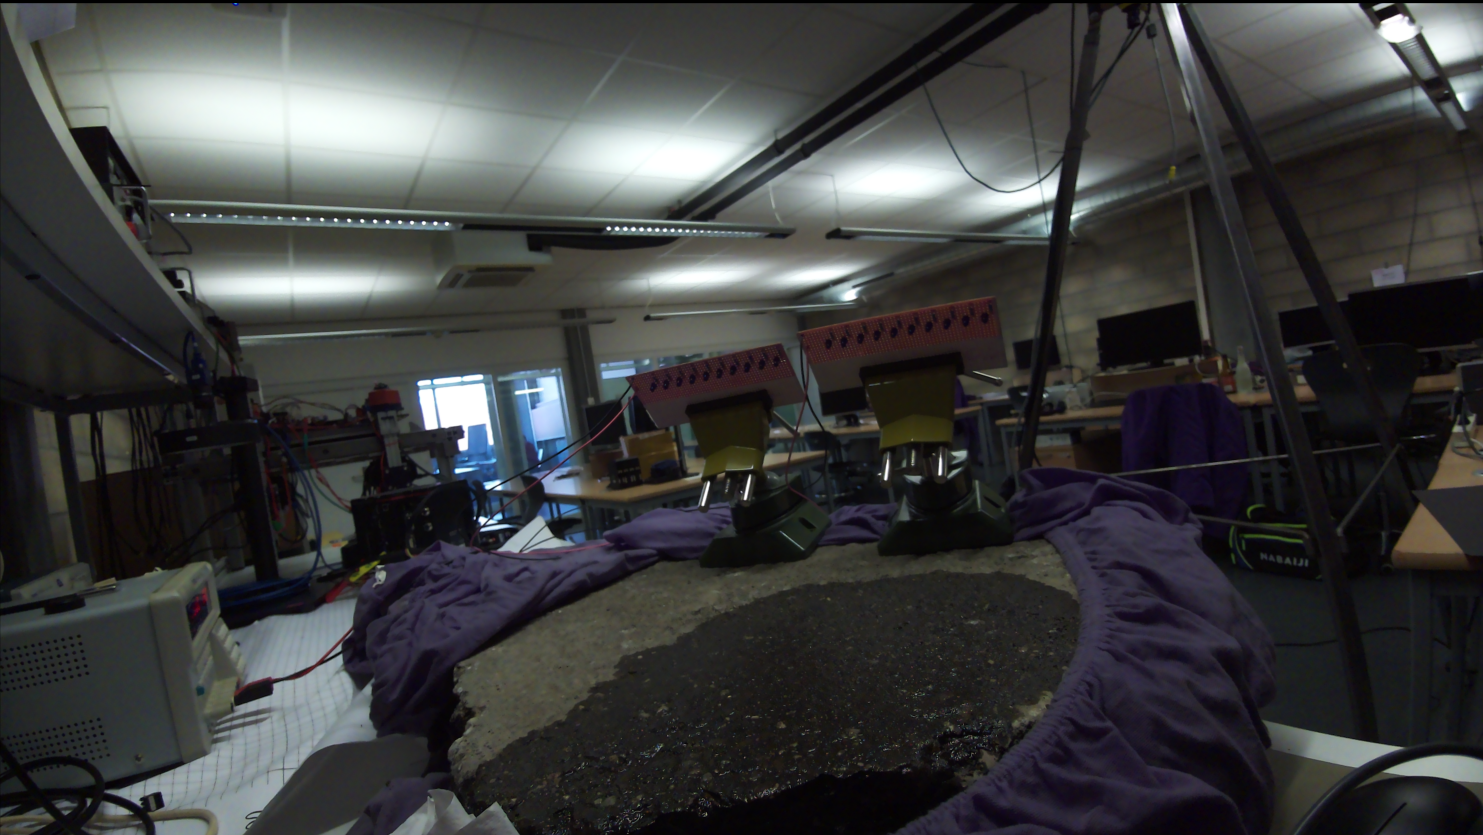
\includegraphics[width=13cm]{assets/figures/camera_vue_couleur1.png}
    \caption{Capture de test - Vue de la scène en couleur}
\end{figure}

Au moment d'effectuer les tests de sensibilités aux IR, tout le matériel n'était pas encore arrivé, notement le filtre de l'objectif ne
laissant passer que les infrarouges. J'ai donc effectué les captures qui vont suivre dans les conditions suivantes:
\begin{itemize}
    \item Lumières éteintes dans la pièce.
    \item Deux lignes de 10 leds IR éclairant en direction de la tâche d'huile de moteur.
    \item Protection contre les lumières parasites du couloir (carton).
    \item Auto-focus sur le centre de l'image
    \item Temps d'exposition: 5000[ns]. (déterminé expérimentalement avec plusieurs captures)
\end{itemize}
Avec ce setup, j'ai effectué plusieurs captures en faisant varier la position de l'éclairage par rapport à la tâche d'huile et la caméra.
J'ai obtenu différents résultats, plus ou moins utilisables.


Ci-dessous, un exemple d'éclairage orienté "contre" la caméra selon la figure suivante:
\begin{figure}[H]
    \centering
    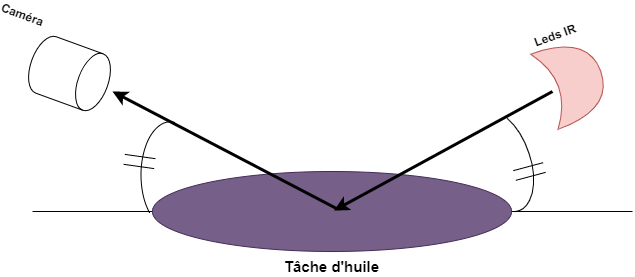
\includegraphics[width=13cm]{assets/figures/eclairage_contre_camera.png}
    \caption{Schéma de capture - Eclairage contre la camera}
\end{figure}


\begin{figure}[H]
    \centering
    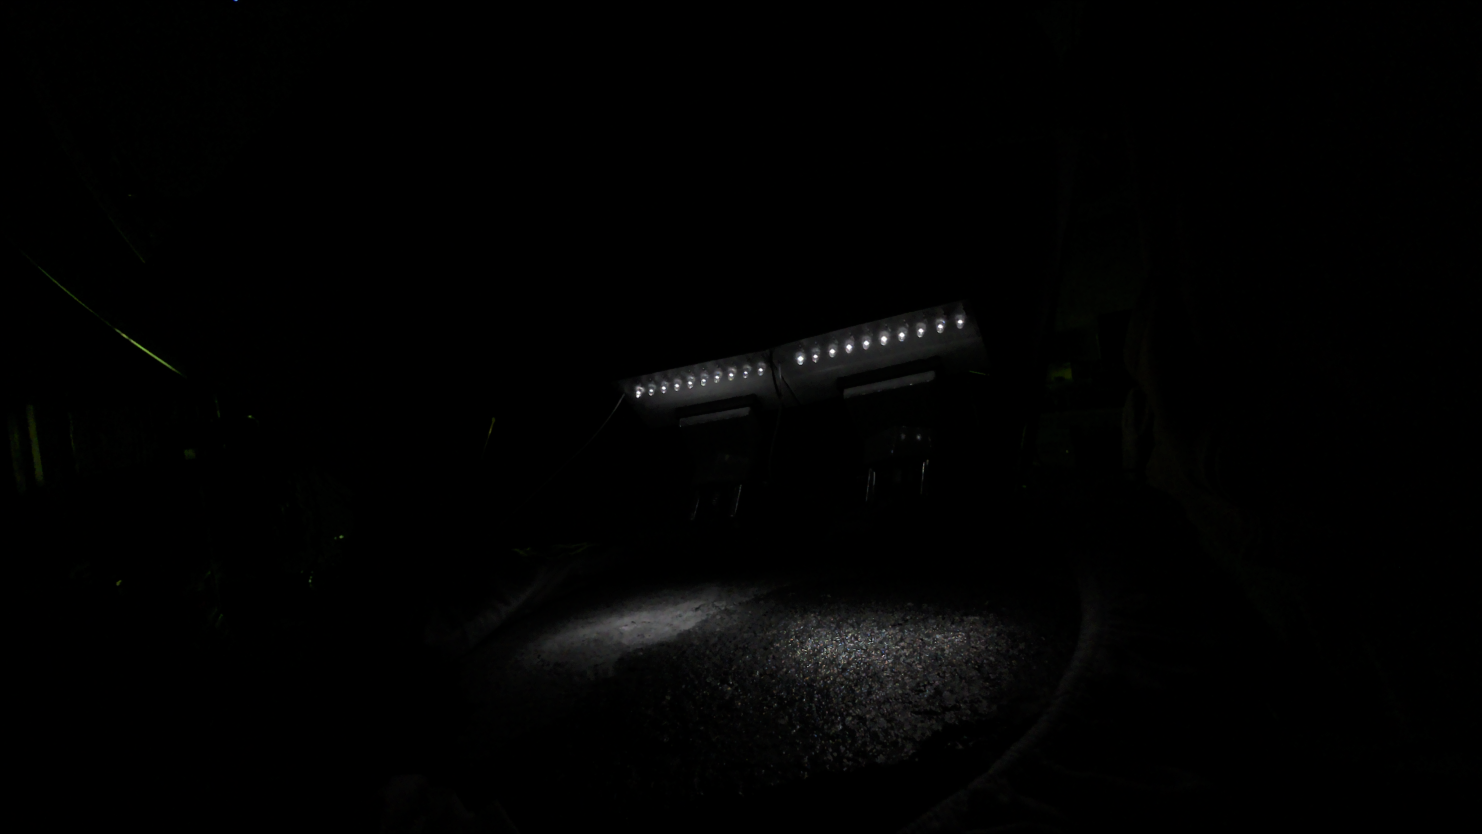
\includegraphics[width=13cm]{assets/figures/eclairage_face1.png}
    \caption{Capture de test - éclairage de face 1}
\end{figure}
\begin{figure}[H]
    \centering
    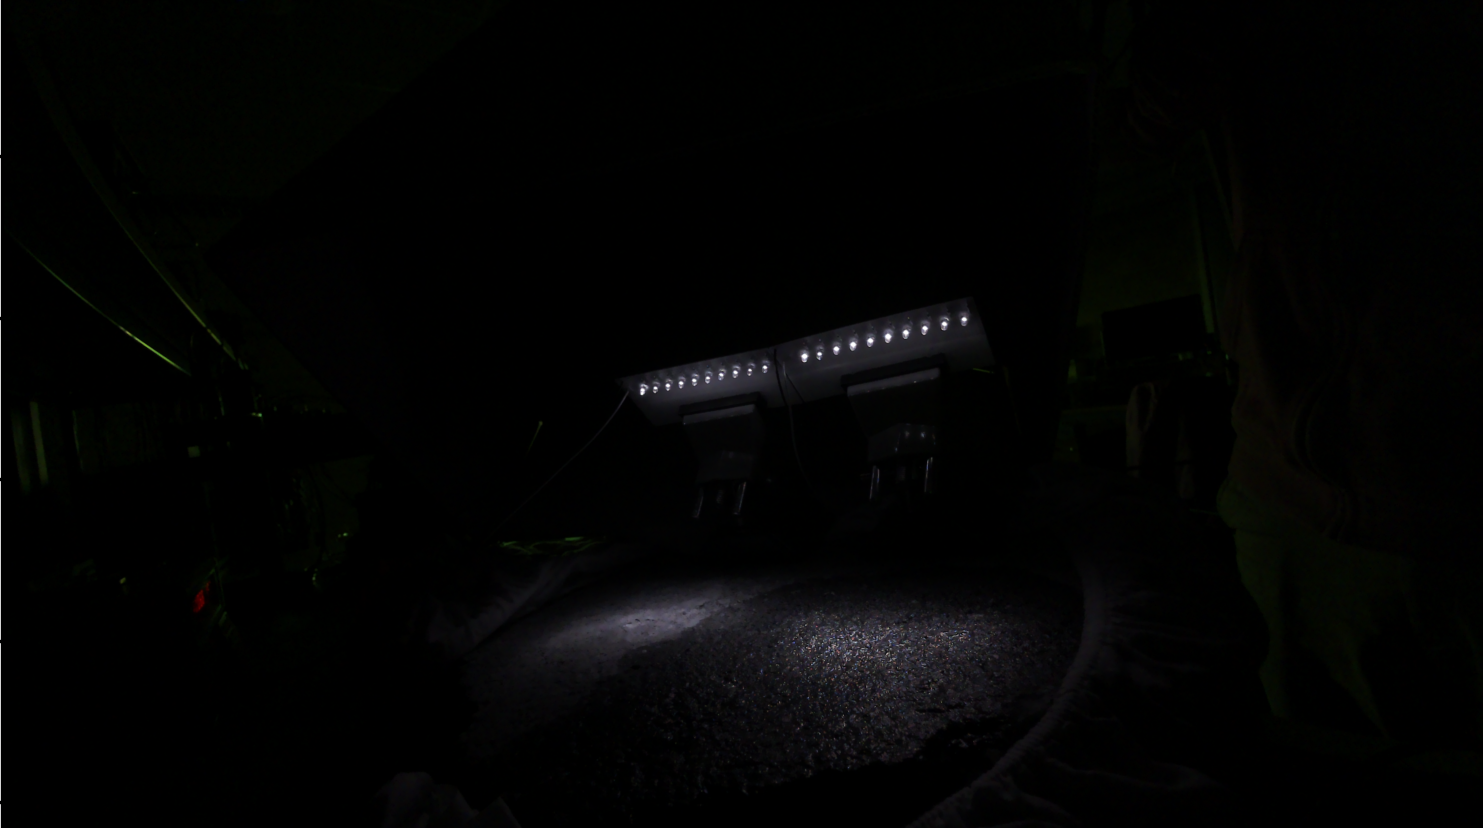
\includegraphics[width=13cm]{assets/figures/eclairage_face2.png}
    \caption{Capture de test - éclairage de face 2}
\end{figure}

On observe que la route et l'huile reflètent les leds IR, à l'oeil nu la différence est notable, mais l'analyse avec un soft peut s'avérer compliquée.\\
Ci-dessous, un exemple d'éclairage orienté perpendiculairement à la route selon la figure suivante:
\begin{figure}[H]
    \centering
    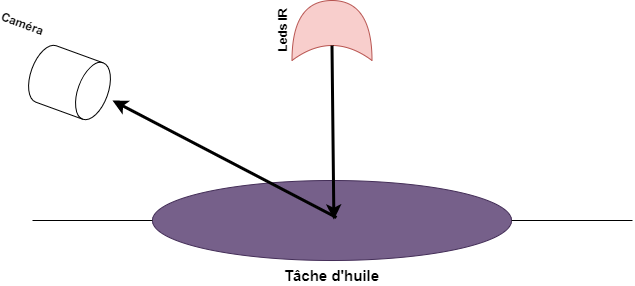
\includegraphics[width=13cm]{assets/figures/eclairage_perpendiculaire.png}
    \caption{Schéma de capture - Eclairage perpendiculaire à la route}
\end{figure}

\begin{figure}[H]
    \centering
    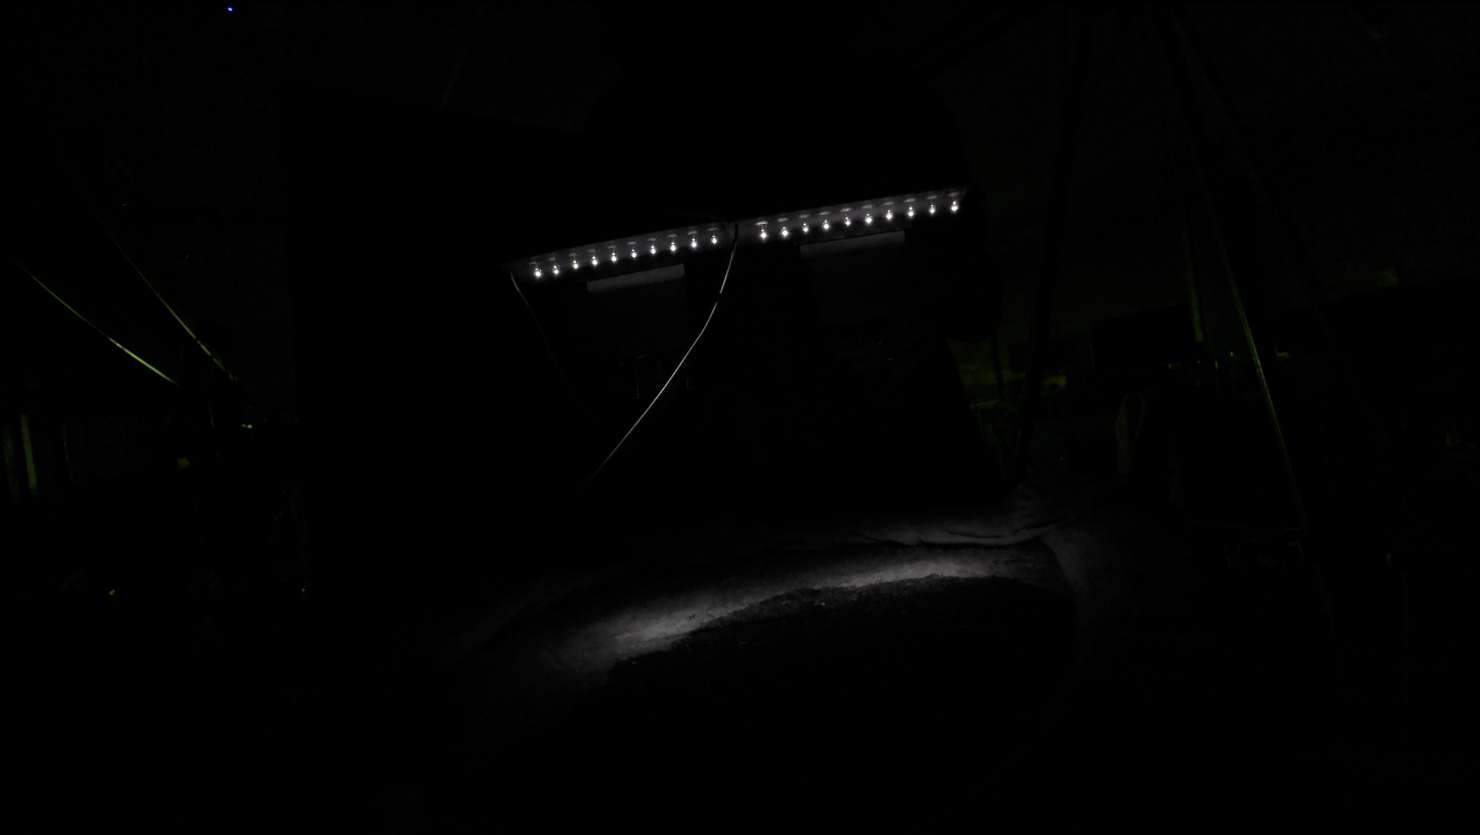
\includegraphics[width=13cm]{assets/figures/eclairage_perpendiculaire1.png}
    \caption{Capture de test - Eclairage perpendiculaire 1}
\end{figure}

\begin{figure}[H]
    \centering
    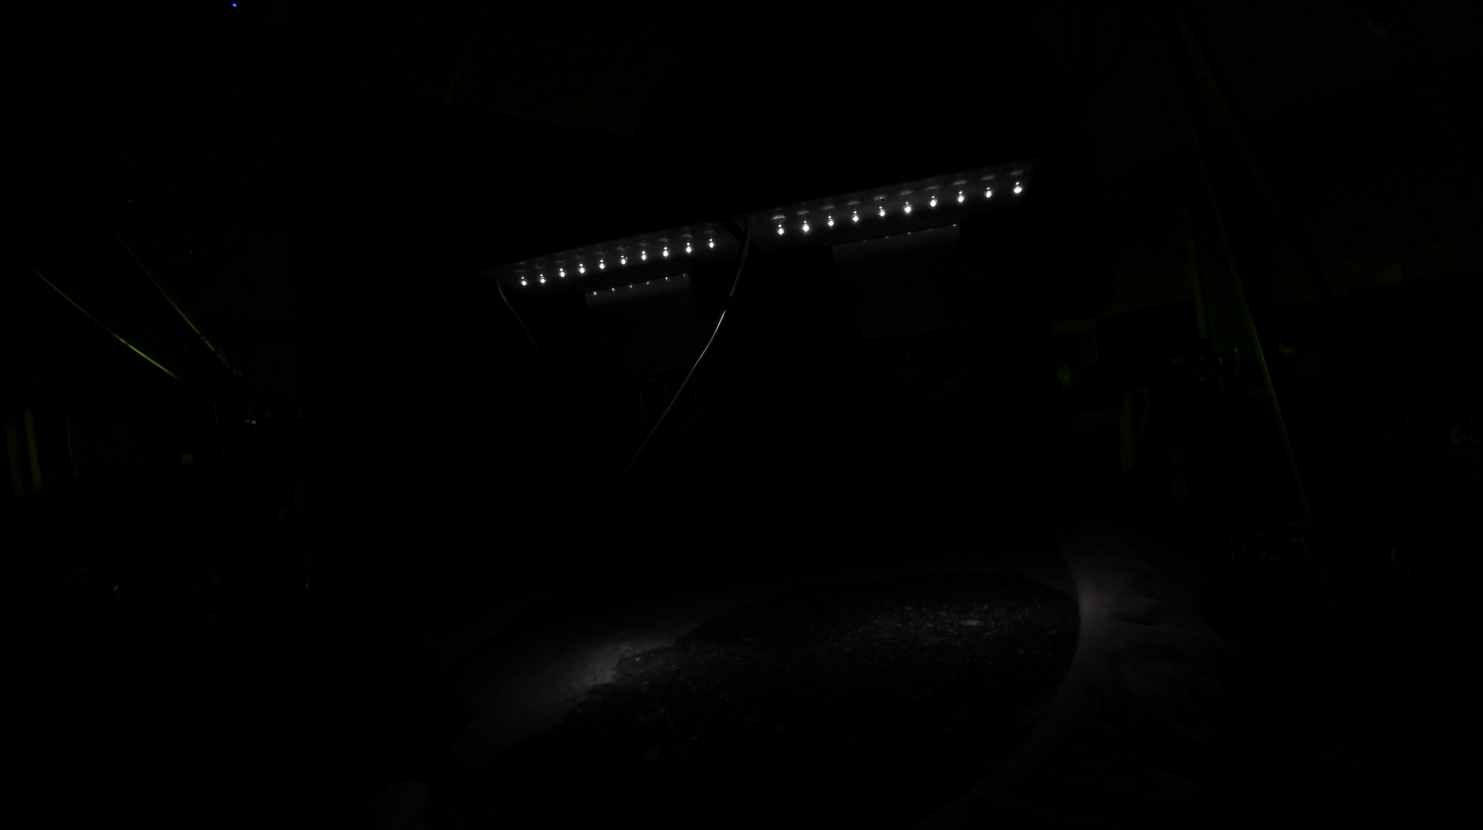
\includegraphics[width=13cm]{assets/figures/eclairage_perpendiculaire2.png}
    \caption{Capture de test - Eclairage perpendiculaire 2}
\end{figure}

\begin{figure}[H]
    \centering
    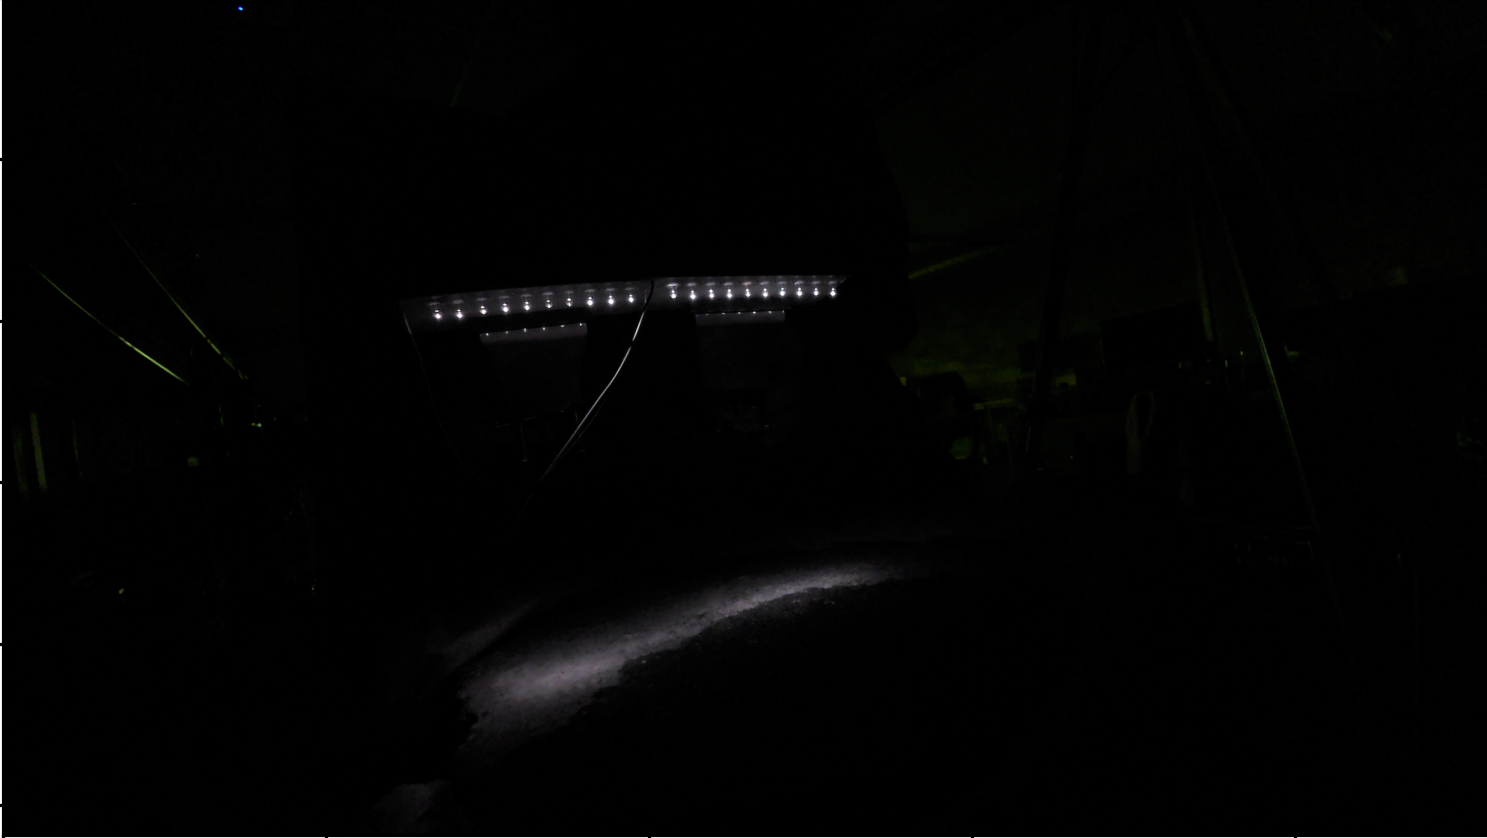
\includegraphics[width=13cm]{assets/figures/eclairage_perpendiculaire3.png}
    \caption{Capture de test - Eclairage perpendiculaire 3}
\end{figure}
On observe que la route diffuse, dans une moindre mesure, l'éclairage des leds IR, là ou l'huile semble absorber les rayonnements. On arrive
assez facilement à différencier le clair de la route et le foncé de l'huile. La mise en place d'un software de détection est envisageable avec
un éclairage basé sur ce schéma. A noté que les tests ont été effectué avec plusieurs gammes de leds (830nm, 850nm et 880nm), la différence
sur le retour image n'est pas très grandes, mais les leds 850nm permettent de mieux différencier la route de l'huile.

[Faire un test avec l'éclairage derrière la caméra]

\section{Installation}
\subsection{Eclairage}

\subsection{Caméra}

\section{Programme}
\subsection{Traitement de l'image}
\subsection{Communication}
